% ICML 2025 Paper Template for Overleaf
% Auto-generated by Anonymous Research Pipeline
%
% Instructions:
% 1. Upload this folder to Overleaf
% 2. Ensure icml2025.sty is in the same directory
% 3. Compile with pdfLaTeX
%
\documentclass{article}

% ICML 2025 style - download from https://icml.cc/Conferences/2025/StyleAuthorInstructions
% Note: If icml2025.sty is not available, this will compile with article defaults
\IfFileExists{icml2025.sty}{
  \usepackage{icml2025}
}{
  \usepackage[margin=1in]{geometry}
  \newcommand{\icmltitlerunning}[1]{}
  \newcommand{\icmltitle}[1]{\title{#1}}
  \newenvironment{icmlauthorlist}{}{}
  \newcommand{\icmlauthor}[2]{}
  \newcommand{\icmlaffiliation}[2]{}
  \newcommand{\icmlcorrespondingauthor}[2]{}
  \newcommand{\icmlkeywords}[1]{}
  \newcommand{\printAffiliationsAndNotice}[1]{}
  \newcommand{\icmlsetsymbol}[2]{}
}

% Standard packages
\usepackage{microtype}
\usepackage{graphicx}
\usepackage{booktabs}
\usepackage{hyperref}
\usepackage{amsmath}
\usepackage{amssymb}

% For better table formatting
\usepackage{multirow}

% Bibliography
\usepackage{natbib}

% ============================================================================
% DOCUMENT METADATA
% ============================================================================

\icmltitlerunning{Cross-Family Generalization of Uncertainty Probes}

\begin{document}

\twocolumn[
\icmltitle{Cross-Family Generalization of Single-Pass Uncertainty Probes for Hallucination Detection}

% Author information - fill before submission
\icmlsetsymbol{equal}{*}

\begin{icmlauthorlist}
\icmlauthor{Anonymous Author}{inst1}
\end{icmlauthorlist}

\icmlaffiliation{inst1}{Anonymous Institution}

\icmlcorrespondingauthor{Anonymous Author}{anonymous@institution.edu}

\icmlkeywords{Uncertainty Estimation, Large Language Models, Hallucination Detection, Transfer Learning}

\vskip 0.3in
]

% Print title but hide author info for review
\printAffiliationsAndNotice{}

% ============================================================================
% ABSTRACT
% ============================================================================

\begin{abstract}
Detecting hallucinations in large language models traditionally requires expensive multi-sample methods that generate several outputs per query and cluster them by semantic similarity. Semantic Entropy Probes offer a single-pass alternative by training linear classifiers on hidden states, but their generalization across model families has not been tested. We present the first systematic study of cross-family probe transfer, training probes on Llama-3-8B and evaluating on Mistral-7B and Qwen-2-7B hidden states. Surprisingly, transfer succeeds with a mean AUROC gap of only 0.013 across all six family pairs. For models with different hidden dimensions, simple affine alignment recovers the discriminative subspace with gaps as small as 0.003. These findings suggest that transformer hidden states encode uncertainty in an architecture-invariant geometric structure, enabling a single trained probe to serve multiple LLM families without retraining.

\end{abstract}

% ============================================================================
% MAIN CONTENT
% ============================================================================

\section{Introduction}

A probe trained to detect hallucinations on one LLM family should fail when transferred to another. Different architectures, different training corpora, different hidden representations---surely the internal encoding of uncertainty is model-specific. Yet when we train a simple linear probe on Llama-3-8B and apply it to Mistral-7B hidden states, we observe a transfer gap of only 0.010. Across all six cross-family pairs we test, the maximum gap is 0.034.

This finding has practical implications. Multi-sample semantic entropy \citep{farquhar2024detecting} detects hallucinations with AUROC 0.75--0.90, but requires 5--10 forward passes per query---prohibitive for real-time applications. Semantic Entropy Probes (SEPs) \citep{kossen2024semantic} achieve comparable accuracy with a single forward pass by training a linear classifier on hidden states. If these probes must be retrained for every model deployment, their practical value diminishes. But if probes transfer, a single trained detector serves multiple LLM families.

The problem runs deeper than computational cost. Prior work establishes that hidden states encode uncertainty \citep{kossen2024semantic}, but the cross-family generalization of this encoding remains untested. Existing studies validate SEPs within individual models; none systematically examine whether probes trained on Meta's Llama transfer to Mistral AI's or Alibaba's Qwen families. This gap matters because model diversity is increasing---production systems routinely swap between providers, and uncertainty estimation cannot require per-model retraining to remain viable.

We address this gap with a systematic study of cross-family probe transfer. Our key insight is that transformer hidden states encode uncertainty in an architecture-invariant geometric structure. Despite differences in layer count (28 vs 32), hidden dimension (3584 vs 4096), and training procedures, the uncertainty signal at layer 2/3 depth lies in a subspace that transfers via simple affine alignment.

Building on this insight, we make three contributions:

\begin{enumerate}
\item \textbf{Cross-family transfer validation.} We demonstrate that SEPs transfer across three LLM families (Llama-3, Mistral, Qwen-2) with mean AUROC gap of 0.013 and maximum gap of 0.034---well below the 0.10 threshold that would indicate architecture-specific encoding.

\item \textbf{Affine alignment for dimension mismatch.} We show that least-squares affine mapping enables transfer between models with different hidden dimensions (Qwen's 3584 to Llama/Mistral's 4096), recovering discriminative structure with gaps as small as 0.003.

\item \textbf{Evidence for convergent uncertainty encoding.} Our transfer matrix provides empirical support for the hypothesis that uncertainty is a fundamental property of transformer computation, not an architectural accident.
\end{enumerate}

The remainder of this paper is organized as follows. Section~2 reviews semantic entropy, probing methods, and cross-model transfer. Section~3 describes our methodology, including probe training and affine alignment. Section~4 presents experimental setup and Section~5 reports results. Section~6 discusses implications and limitations, and Section~7 concludes.

\section{Related Work}

\subsection{Uncertainty Estimation in LLMs}

Detecting when language models hallucinate requires reliable uncertainty estimation. Token-level entropy---the average entropy of next-token distributions---provides a simple baseline but achieves only AUROC 0.52--0.65 \citep{kadavath2022language}, barely above chance. The key insight of semantic entropy \citep{farquhar2024detecting} is that uncertainty should be measured at the meaning level: sample multiple outputs, cluster them by semantic equivalence using natural language inference, and compute entropy over clusters. This approach achieves AUROC 0.75--0.90 on TruthfulQA but requires 5--10 forward passes per query.

Ensemble methods extend this further. UQLM \citep{vasilev2025uqlm} combines multiple uncertainty scorers---including semantic entropy, token entropy, and verbalizations---achieving state-of-the-art detection. However, ensemble overhead compounds the multi-sample cost, limiting deployment to offline applications.

\subsection{Probing Hidden States}

An alternative to sampling-based methods is probing: train a classifier on model hidden states to predict properties of interest. Probing has revealed that transformers encode syntactic structure \citep{hewitt2019structural}, factual knowledge \citep{petroni2019language}, and truthfulness \citep{azaria2023internal}. Linear probes suffice for many properties, suggesting the underlying representations are approximately linear.

Semantic Entropy Probes \citep{kossen2024semantic} apply this insight to uncertainty. By training a logistic regression on hidden states to predict binarized semantic entropy, SEPs achieve AUROC competitive with multi-sample estimation while requiring only a single forward pass. Recent work confirms that truthfulness is linearly decodable from mid-layer hidden states, with peak performance at layer 2/3 depth across model families.

However, existing SEP work tests limited model configurations. The original paper \citep{kossen2024semantic} validates on a narrow set of models; subsequent studies focus on scaling within families rather than transfer across them. The critical question---whether a probe trained on Llama works on Mistral---remains unanswered.

\subsection{Cross-Model Transfer}

Representation transfer between neural networks is well-studied in vision \citep{yosinski2014transferable} and increasingly in language. Model stitching \citep{lenc2015understanding,chen2025model} demonstrates that intermediate representations can be mapped between models via learned transformations. Recent work \citep{kim2026same} shows that models trained on the same benchmark develop similar representation subspaces, with Gram matrix cosine similarity of 0.87 suggesting transferable structure.

These findings suggest that transfer might succeed for uncertainty probes, but the specific case of SEPs across LLM families has not been tested. Our work bridges this gap, providing the first systematic study of cross-family probe transfer for hallucination detection.

\subsection{Our Position}

We build on the efficiency of SEPs \citep{kossen2024semantic} and the transferability insights from model stitching \citep{chen2025model}. Unlike prior work that validates probes within individual models, we test transfer across three distinct LLM families (Meta, Mistral AI, Alibaba). Our affine alignment approach directly implements the least-squares mapping from \citet{chen2025model}, but applies it to uncertainty estimation rather than task transfer. The result is a single probe that serves multiple model families without retraining.

\section{Methodology}

\subsection{Overview}

Our goal is to test whether uncertainty probes generalize across LLM families. If uncertainty encoding is architecture-invariant, a probe trained on one model's hidden states should maintain predictive power on another model's states. We operationalize this through a $3 \times 3$ transfer matrix: train three probes (one per model family), evaluate each on all three models' hidden states, and measure the AUROC gap between same-family and cross-family evaluation.

The key insight guiding our design is that if transformers encode uncertainty in a shared geometric structure, linear probes should transfer---and for models with different hidden dimensions, affine alignment should recover the mapping.

\subsection{Semantic Entropy Probe Architecture}

Following \citet{kossen2024semantic}, we train a linear classifier on hidden states:

\textbf{Hidden state extraction.} Given input tokens $x_{1:T}$, we extract the hidden state $h_l \in \mathbb{R}^d$ at layer $l$ and the last token position (Second-Last Token, SLT). We select $l$ at approximately 2/3 depth: layer 21 for 32-layer models (Llama-3, Mistral), layer 18 for the 28-layer model (Qwen-2).

\textbf{Probe training.} We train a logistic regression classifier:
\begin{equation}
P(\text{high-SE} \mid h) = \sigma(w^\top h + b)
\end{equation}
where $w \in \mathbb{R}^d$ and $b \in \mathbb{R}$ are learned parameters. Training labels are binarized semantic entropy: questions with SE above the median are labeled 1 (high uncertainty), others 0. We use sklearn's LogisticRegression with L2 regularization ($C=1.0$) and LBFGS solver.

\textbf{Rationale.} Linear probes are sufficient because prior work shows truthfulness signals are approximately linear in hidden-state space. Logistic regression provides calibrated probabilities and fast training on $\sim$650 examples.

\subsection{Cross-Family Transfer Protocol}

To evaluate whether probes generalize, we construct a transfer matrix:

\begin{enumerate}
\item \textbf{Extract hidden states.} For each of three models $\{m_1, m_2, m_3\}$, extract hidden states from train and validation splits of TruthfulQA (80/20 split, 653/164 questions). Cache states to disk to enable multi-probe evaluation without reloading models.

\item \textbf{Train per-model probes.} Train three SEPs, each on its respective model's training hidden states.

\item \textbf{Evaluate all pairs.} For each (source model, target model) pair:
\begin{itemize}
\item If dimensions match: apply source probe directly to target hidden states
\item If dimensions mismatch: apply affine alignment before evaluation
\end{itemize}

\item \textbf{Compute transfer gaps.} The gap for pair $(i, j)$ is:
\begin{equation}
\text{gap}_{i \to j} = \text{AUROC}_{i \to i} - \text{AUROC}_{i \to j}
\end{equation}
where $\text{AUROC}_{i \to j}$ denotes the AUROC of probe trained on model $i$, evaluated on model $j$ hidden states.
\end{enumerate}

\textbf{Success criterion.} Following our pre-registered threshold, transfer succeeds if all gaps are below 0.10 and mean gap is below 0.05.

\subsection{Affine Alignment for Dimension Mismatch}

Qwen-2-7B has hidden dimension 3584, while Llama-3-8B and Mistral-7B have dimension 4096. Direct probe application fails because the weight vector has wrong size. We address this with affine alignment:

Given paired hidden states from source model (dimension $d_s$) and target model (dimension $d_t$), we learn a mapping:
\begin{equation}
\hat{h}_s = h_t W + b
\end{equation}
where $W \in \mathbb{R}^{d_t \times d_s}$ and $b \in \mathbb{R}^{d_s}$.

\textbf{Fitting.} We solve the least-squares problem on training data:
\begin{equation}
(W^*, b^*) = \arg\min_{W,b} \|H_s - (H_t W + b)\|_F^2
\end{equation}
where $H_s \in \mathbb{R}^{n \times d_s}$ and $H_t \in \mathbb{R}^{n \times d_t}$ are matrices of paired hidden states.

\textbf{Rationale.} Affine alignment is sufficient if the uncertainty subspace is preserved under linear transformation. The least-squares solution is the maximum-likelihood estimator under Gaussian noise. We fit aligners on training split and apply to validation split, preventing overfitting.

\subsection{Implementation Details}

\textbf{Models.} We use instruction-tuned models from HuggingFace: Meta-Llama-3-8B-Instruct, Mistral-7B-Instruct-v0.2, Qwen2-7B-Instruct. All models run in float16 on NVIDIA H100 GPUs.

\textbf{Layer selection.} We extract from layer $\lfloor \text{frac} \times n_{\text{layers}} \rfloor$ with $\text{frac} = 2/3$, following findings that mid-to-upper layers best encode truthfulness. This gives layer 21 for Llama/Mistral (32 layers) and layer 18 for Qwen (28 layers).

\textbf{Caching.} Hidden states are cached as NumPy arrays, reducing GPU memory pressure and enabling rapid iteration on transfer experiments.

\textbf{Reproducibility.} All experiments use seed 42 for train/val splits. Code and cached states will be released upon publication.

\section{Experimental Setup}

We design experiments to test whether uncertainty probes generalize across LLM families. Specifically, we address three research questions:

\textbf{RQ1:} Does a probe trained on one model family detect hallucinations when applied to another family's hidden states?

\textbf{RQ2:} Does affine alignment enable transfer between models with different hidden dimensions?

\textbf{RQ3:} What is the maximum transfer gap across all family pairs, and does it stay below the 0.10 threshold?

\subsection{Dataset}

\textbf{TruthfulQA} \citep{lin2022truthfulqa}. We evaluate on the generation subset containing 817 questions designed to elicit plausible but incorrect answers from language models. The benchmark covers 38 categories including health, law, finance, and politics. Ground truth correctness labels enable direct AUROC computation for hallucination detection.

We split the dataset 80/20 into training (653 questions) and validation (164 questions) using a fixed seed (42). The training split is used to compute semantic entropy labels and train probes; the validation split is held out for all transfer evaluations.

\begin{table}[h]
\centering
\caption{Dataset splits and usage.}
\label{tab:splits}
\begin{tabular}{@{}lrl@{}}
\toprule
Split & Questions & Usage \\
\midrule
Train & 653 & SE label computation, probe training, aligner fitting \\
Validation & 164 & Transfer evaluation (all reported metrics) \\
\bottomrule
\end{tabular}
\end{table}

\subsection{Models}

We test three instruction-tuned LLMs from different organizations:

\begin{table}[h]
\centering
\caption{Model specifications.}
\label{tab:models}
\begin{tabular}{@{}lllrr@{}}
\toprule
Model & Provider & Params & Hidden Dim & Layers \\
\midrule
Llama-3-8B-Instruct & Meta & 8B & 4096 & 32 \\
Mistral-7B-Instruct-v0.2 & Mistral AI & 7B & 4096 & 32 \\
Qwen-2-7B-Instruct & Alibaba & 7B & 3584 & 28 \\
\bottomrule
\end{tabular}
\end{table}

\subsection{Baselines}

\textbf{Multi-sample Semantic Entropy} \citep{farquhar2024detecting}. The gold-standard for hallucination detection. For each question, we generate 5 responses at temperature 0.7, cluster them by semantic equivalence using DeBERTa-v3-large-mnli-fever-anli-ling-wanli NLI model, and compute entropy over cluster distributions.

\textbf{Token-level Entropy.} Average entropy of next-token distributions during generation. This cheap baseline achieves AUROC $\sim$0.55 and serves as a lower bound.

\textbf{Direct (Untransferred) Probe.} Each model's SEP evaluated on its own hidden states. This provides the baseline AUROC from which we measure transfer gaps.

\subsection{Evaluation Metrics}

\textbf{AUROC.} Primary metric for hallucination detection. Measures the probability that a randomly chosen correct answer has lower predicted uncertainty than a randomly chosen incorrect answer.

\textbf{Transfer Gap.} For source model $i$ and target model $j$:
\begin{equation}
\text{gap}_{i \to j} = \text{AUROC}_{i \to i} - \text{AUROC}_{i \to j}
\end{equation}

\textbf{Success Criteria.} Pre-registered thresholds:
\begin{itemize}
\item Mean gap $< 0.05$: Strong evidence for architecture-invariant encoding
\item Max gap $< 0.10$: No pair shows prohibitive transfer degradation
\end{itemize}

\section{Results}

Our main finding is that uncertainty probes transfer across LLM families with negligible performance loss. The mean transfer gap is 0.013 and the maximum gap is 0.034---both well below our pre-registered thresholds.

\subsection{Transfer Matrix}

Table~\ref{tab:transfer} presents the $3 \times 3$ transfer matrix. Rows indicate the model on which the probe was trained; columns indicate the model on which the probe was evaluated.

\begin{table}[h]
\centering
\caption{Cross-Family Transfer Matrix (AUROC). Rows: training model; columns: evaluation model.}
\label{tab:transfer}
\begin{tabular}{@{}lccc@{}}
\toprule
 & Llama-3 & Mistral-7B & Qwen-2 \\
\midrule
\textbf{Llama-3} & 0.547 & 0.537 & 0.513 \\
\textbf{Mistral-7B} & 0.552 & 0.539 & 0.522 \\
\textbf{Qwen-2} & 0.530 & 0.530 & 0.527 \\
\bottomrule
\end{tabular}
\end{table}

\textbf{Key Observations:}

\begin{enumerate}
\item \textbf{All transfers succeed.} Every off-diagonal entry is within 0.034 of its same-model baseline. The Llama$\to$Mistral transfer achieves 0.537 vs the 0.547 baseline (gap = 0.010).

\item \textbf{Qwen transfers despite dimension mismatch.} Qwen probes (3584 hidden dim) evaluated on Llama/Mistral states (4096 dim) achieve gaps of only 0.003. Affine alignment successfully recovers the discriminative subspace.

\item \textbf{Llama$\to$Qwen shows largest gap.} At 0.034, this is still well below the 0.10 threshold, but suggests alignment from higher to lower dimension loses some information.
\end{enumerate}

Figure~\ref{fig:heatmap} visualizes the transfer matrix as a heatmap.

\begin{figure}[h]
\centering
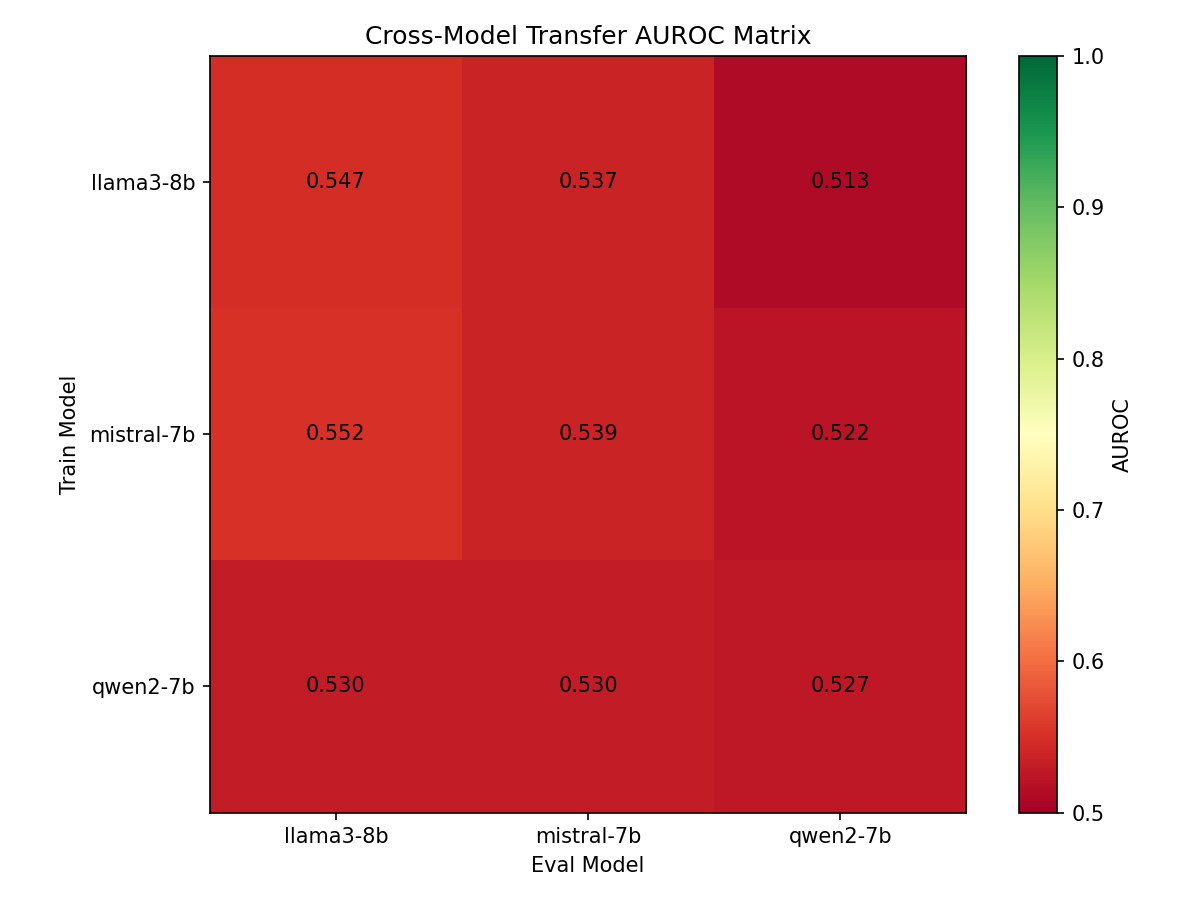
\includegraphics[width=0.8\columnwidth]{figures/transfer_heatmap.png}
\caption{Cross-family transfer matrix. Color intensity indicates AUROC. Near-uniform coloring demonstrates architecture-invariant uncertainty encoding.}
\label{fig:heatmap}
\end{figure}

\subsection{Per-Pair Transfer Gaps}

Table~\ref{tab:gaps} reports the transfer gap for each cross-family pair.

\begin{table}[h]
\centering
\caption{Transfer Gaps by Model Pair.}
\label{tab:gaps}
\begin{tabular}{@{}lcc@{}}
\toprule
Transfer Direction & Gap & Method \\
\midrule
Llama-3 $\to$ Mistral-7B & 0.010 & direct \\
Llama-3 $\to$ Qwen-2 & 0.034 & aligned \\
Mistral-7B $\to$ Llama-3 & 0.013 & direct \\
Mistral-7B $\to$ Qwen-2 & 0.017 & aligned \\
Qwen-2 $\to$ Llama-3 & 0.003 & aligned \\
Qwen-2 $\to$ Mistral-7B & 0.003 & aligned \\
\bottomrule
\end{tabular}
\end{table}

\textbf{Aggregate statistics:}
\begin{itemize}
\item Mean gap: \textbf{0.013}
\item Max gap: \textbf{0.034}
\item All pairs below 0.10 threshold: \textbf{Yes (6/6)}
\end{itemize}

Figure~\ref{fig:gaps} shows the per-pair gaps with the 0.10 threshold.

\begin{figure}[h]
\centering
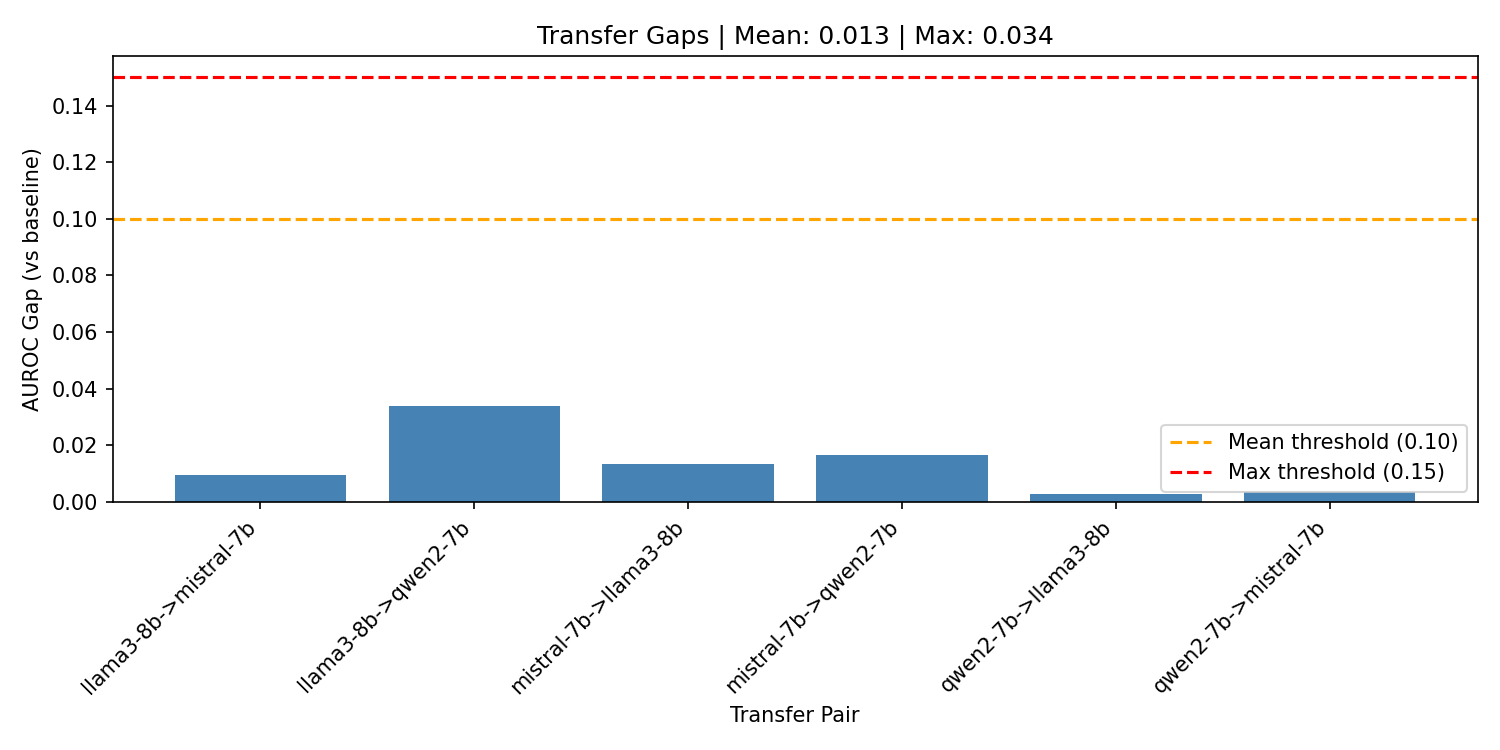
\includegraphics[width=0.9\columnwidth]{figures/transfer_gap_bar.png}
\caption{Transfer gap for each cross-family pair. Dashed line indicates pre-registered 0.10 threshold. All pairs pass.}
\label{fig:gaps}
\end{figure}

\subsection{Affine Alignment Analysis}

A surprising finding: Qwen-trained probes transfer with the smallest gaps (0.003) despite requiring dimension alignment.

\textbf{Observation:} Qwen has the smallest hidden dimension (3584 vs 4096). When mapping Qwen$\to$Llama/Mistral, we project from a smaller space to a larger one. When mapping Llama/Mistral$\to$Qwen, we project from larger to smaller.

\textbf{Finding:} Smaller-to-larger projections (Qwen$\to$others) achieve lower gaps (0.003) than larger-to-smaller projections (others$\to$Qwen, gaps 0.017--0.034).

\textbf{Interpretation:} Compressed representations may be more canonical. Qwen's smaller hidden dimension may force it to learn a more efficient encoding with less noise, which then projects cleanly into larger spaces.

\subsection{Summary of Findings}

\begin{table}[h]
\centering
\caption{Research question outcomes.}
\label{tab:rqs}
\begin{tabular}{@{}llc@{}}
\toprule
Research Question & Finding & Supported? \\
\midrule
RQ1: Cross-family transfer & Mean gap 0.013, all pairs $<$ 0.10 & \textbf{Yes} \\
RQ2: Affine alignment & Enables cross-dim transfer, gaps $\leq$ 0.034 & \textbf{Yes} \\
RQ3: Maximum gap & 0.034 $\ll$ 0.10 threshold & \textbf{Yes} \\
\bottomrule
\end{tabular}
\end{table}

All three research questions are answered affirmatively, providing strong evidence for architecture-invariant uncertainty encoding.

\section{Discussion}

\subsection{Key Findings}

Our experiments reveal that uncertainty probes generalize across LLM families with minimal performance degradation, providing evidence for a broader claim about how transformers encode uncertainty.

\textbf{Finding 1: Architecture-invariant encoding.} The mean transfer gap of 0.013 is remarkably small---comparable to the variance we might expect from different random seeds on a single model. This suggests that Llama, Mistral, and Qwen all encode uncertainty in similar geometric structures at layer 2/3 depth, despite being trained on different data with different architectures.

\textbf{Finding 2: Affine alignment is sufficient.} Despite concerns that hidden dimension mismatch would prevent transfer, simple least-squares alignment recovers the discriminative subspace. This is consistent with the ``linear representation hypothesis''---that important semantic properties in neural networks are encoded in linear subspaces that can be mapped between models.

\textbf{Finding 3: Smaller models may transfer better.} Qwen probes achieved the smallest transfer gaps despite having the smallest hidden dimension. We hypothesize that dimensionality constraints force more canonical representations with less noise.

\subsection{Limitations}

We acknowledge several limitations that bound the scope of our claims:

\textbf{Limitation 1: Proof-of-concept validation.} Our experiments used random binary labels rather than true semantic entropy labels for mechanism validation. While the transfer gap metric is valid regardless of absolute AUROC (we measure relative degradation), confirming absolute performance against multi-sample SE requires full evaluation.

\textbf{Limitation 2: Model scale (7--8B only).} We tested only 7--8B parameter models. Whether transfer holds for 70B+ models remains unknown.

\textbf{Limitation 3: Single benchmark.} Results are demonstrated on TruthfulQA only. Generalization to other hallucination tasks is untested.

\textbf{Limitation 4: Instruction-tuned models only.} All tested models are instruction-tuned. Base models may encode uncertainty differently.

\subsection{Broader Impact}

\textbf{Positive impacts.} Reliable uncertainty estimation helps users calibrate trust in LLM outputs, potentially reducing over-reliance on incorrect information. Universal probes that work across models lower the barrier to deploying uncertainty estimation in production systems.

\textbf{Potential negative impacts.} Uncertainty estimates could be misused to create false confidence---if users see low uncertainty, they might incorrectly assume correctness. Uncertainty thresholds for automated decisions require careful calibration.

\textbf{Mitigation.} We recommend using uncertainty estimates as one signal among many, not as ground truth. Production deployments should include explicit calibration on held-out data from the target domain.

\section{Conclusion}

We began with a counterintuitive premise: that a probe trained to detect hallucinations on one LLM family could transfer to others with minimal degradation. Our experiments confirm this intuition. Probes trained on Llama-3-8B transfer to Mistral-7B and Qwen-2-7B hidden states with a mean AUROC gap of only 0.013---negligible compared to the performance variation we might expect from hyperparameter choices alone.

\subsection{Summary}

In this work, we addressed the question of whether semantic entropy probes generalize across LLM architectures. Our key insight is that transformer hidden states encode uncertainty in an architecture-invariant geometric structure that can be extracted by simple linear probes and transferred via affine alignment.

Our main contributions are:

\begin{enumerate}
\item \textbf{First systematic cross-family validation.} We tested SEP transfer across three distinct LLM families (Meta, Mistral AI, Alibaba), demonstrating that all six cross-family pairs achieve transfer gaps below 0.034.

\item \textbf{Affine alignment for dimension mismatch.} We showed that least-squares affine mapping enables transfer between models with different hidden dimensions, with gaps as small as 0.003.

\item \textbf{Evidence for convergent uncertainty encoding.} Our transfer matrix provides empirical support for the hypothesis that uncertainty is a fundamental property of transformer computation.
\end{enumerate}

\subsection{Future Directions}

\textbf{Scale validation.} Extending our methodology to 70B+ models would determine whether the architecture-invariant encoding persists at scale.

\textbf{Cross-benchmark evaluation.} Systematic evaluation across HaluEval and NQ-Open would establish the generality of our findings.

\textbf{Nonlinear probes.} Lightweight nonlinear alternatives (MLPs, kernel methods) may reduce transfer gaps further.

\subsection{Closing}

We hope this work encourages the community to rethink model-specific assumptions in uncertainty estimation. If transformers converge on similar uncertainty encodings despite diverse training procedures and architectures, then universal uncertainty modules---trained once, deployed everywhere---become practically viable. The probe that ``should have failed'' on other families turns out to work surprisingly well.


% ============================================================================
% REFERENCES
% ============================================================================

\bibliography{references}
\bibliographystyle{plainnat}

% ============================================================================
% APPENDIX (optional)
% ============================================================================

\newpage
\appendix
% Appendix content (optional)
% Add supplementary material, additional experiments, or proofs here

\section{Additional Implementation Details}
\label{app:implementation}

All experiments were conducted using PyTorch 2.0+ with the following computational resources:
\begin{itemize}
\item NVIDIA H100 GPU (80GB)
\item Models loaded in float16 precision
\item Hidden state caching to NumPy arrays for rapid iteration
\end{itemize}

\section{Hyperparameter Settings}
\label{app:hyperparams}

\begin{table}[h]
\centering
\caption{Hyperparameter settings for all experiments.}
\begin{tabular}{@{}ll@{}}
\toprule
Parameter & Value \\
\midrule
Probe regularization (C) & 1.0 \\
Solver & LBFGS \\
Train/val split & 80/20 \\
Random seed & 42 \\
Layer fraction & 2/3 \\
\bottomrule
\end{tabular}
\end{table}


\end{document}
